%!TEX root = ..\..\dissertation.tex
\section{Classification of Production Processes}\label{sec:clsfProc}
\cref{paper:CMS2018} is entitled~\citetitle{SorensenCMS2018}, written for and presented at the 51st CIRP Conference on Manufacturing Systems (CMS2018) in 2018.
It relates to and addresses \cref{resq2} by answering the following sub-question:
\begin{enumerate}[leftmargin=3em, label=RQ2.\arabic*]
    \item How can processes during production of discrete products be classified independently of the means facilitating the process?
\end{enumerate}
The study was carried out as a literature review of production and manufacturing processes.
Through an iterative search and consolidation process, a classification scheme on production processes was created by consolidating existing classification schemes.
The purpose of this was to lay the foundation for making a quantitative and more objective comparison of manufacturing systems, in order to identify potential \gls{glos:platformCand}s.

\subsection{Extended Abstract}
\subsubsection*{Introduction \& Method}
Simultaneous development of products and manufacturing systems based on co-existing platforms of standardised assets has been gaining traction~\parencite{MichaelisJohannesson,ElMaraghy2015407}.
However, development of manufacturing system platforms remains a difficult task~\parencite{BossenPbCd}, with many inherent challenges.
One such challenge is the identification of potential platforms, \ie{} \gls{glos:platformCand}s, based on a company's existing manufacturing systems.
To properly identify platform candidates, a way to consistently identify common processes across manufacturing systems is needed.
This can be achieved through a classification scheme for production processes.
Using the common vocabulary and definitions in a classification scheme, processes, and thus process commonality between systems, can be identified consistently in a standardised manner.
Consistency and standardisation are key aspects of platforms.

Various classification schemes for manufacturing processes or material handling processes exist, and a few include test and inspection processes, but no single classification scheme has been found to incorporate all of these.
Such a consolidated classification scheme could greatly benefit the manufacturing system platform development task by, easing both the collection of data and the identification of commonality in manufacturing systems.
Focus for the consolidated process classification scheme presented in the following is on discrete manufacturing.
While it may have applications outside discrete manufacturing, creating a classification scheme for the process industry poses different challenges, partly due to a prevalence of shapeless materials.

In order to structure the creation of the classification scheme, the study employed an iterative approach switching between searching for and consolidating classification schemes, taxonomies, or ontologies for manufacturing processes and material handling processes.
It is essentially a simplified adaption of the design science research cycles~\parencite{Hevner2007TheTC}.
The first part of the approach was a simple search on a number of keyword combinations followed by pearl-growing.
The consolidation step was focused on grouping processes, process discrepancies (\eg{} included/excluded processes), and how well the classification schemes fit the following criteria:
\begin{itemize}
  \item include both manufacturing and handling processes
  \item clearly differentiable levels
  \item manageable amount of levels
  \item function-based processes
\end{itemize}
Following these criteria, the intention was to create a comprehensive classification scheme that was easily navigable, and consisted of processes independent of the means or equipment performing the processes.
Function-based processes make it easier to identify alternatives to existing solutions, and compare production systems that may not have much similarity in terms of equipment, but rather in the processes they carry out.

\subsubsection*{Classifications \& Taxonomies}
As a basis for categorising manufacturing and material handling processes, this study subscribes to the notion of added \emph{utility} rather than added value \parencite{Kay12MHE,Apple1972}.
Material handling processes add ``time'' and ``place'' utility, by ensuring workpieces are in the right place at the right time, and manufacturing processes add ``form'' utility by changing the shape and composition of a workpiece.
Traditionally, material handling processes are considered non-value-adding processes, but they are still necessary for many value-adding processes to be successful.

To create the consolidated classification scheme, several classifications, taxonomies, and ontologies were reviewed.
Six key schemes form the main influencers of the consolidated classification scheme; four for manufacturing processes~\parencite{DIN8580,Ashby2011,Kalpakjian,9780831130497} and two for material handling processes~\parencite{VDI2860,Kay12MHE}.
None of the six key classification schemes, or any of the additional reviewed schemes, fulfil the first criteria on including both manufacturing and material handling processes, but the consolidated classification scheme does.

A common aspect of the reviewed classification schemes is, that the primary way to categorise manufacturing processes whether they are shaping or non-shaping~\parencite{9780831130497,Ashby2011,DIN8580,Kalpakjian}, \ie{} whether they change the shape of an object or not.
Following this first differentiation, there are a number of ways to categories manufacturing processes.
\textcite{9780831130497} group processes in up to eight levels, making the distinction clear, but difficult to manage in terms of levels.
DIN 8580:2009--09 (henceforth DIN 8580) groups processes according to material state and whether the process creates, reduces, or preserves the coherence of a given workpiece.
This incorporates shaping/non-shaping implicitly, rather than explicitly.
\textcite{Ashby2011} initially groups processes depending on when they occur, \ie{} primary shaping for creating the initial shape of the workpiece, secondary processes for adding features, joining for assembly, and surface treatment for finishing.
Subsequently, the processes are grouped hierarchically into four levels (universe, family, class, and subclass).
\textcite{Kalpakjian} have six families of processes with three levels each, grouping each process' corresponding description according to the material they are applicable to.
In general, as the level of detail increases, the classification of processes becomes more dependent on the means/equipment used to perform the process.

The reviewed material handling classifications are largely equipment-based and defined by the four primary material handling functions described by \textcite{578045219951201}; transport, positioning, unit load formation, and storage.
\textcite{Kay12MHE} adds ``identification and control'' as a fifth category.
VDI 2860:1990--05 (henceforth VDI 2860) breaks material handling into three groups focusing on the ``handling'' processes, and references other standards for the two remaining groups (``transport'' and ``storage(hold)'')~\parencite{VDI2860}.
``Handling'' is broken down an additional two times, reaching elementary functions (\eg{} ``rotate'') and composite functions (\eg{} ``allocate'') at the lowest level.
VDI 2860 also introduces a set of symbols for creating flow charts based on the standard, and is independent of equipment and means.

\subsubsection*{Results}
An overview of the consolidated classification scheme is presented on \cref{fig:clsfScheme}, with a partially expanded view of the ``manufacturing process'' category.
\begin{figure}[tb]
  \centering
  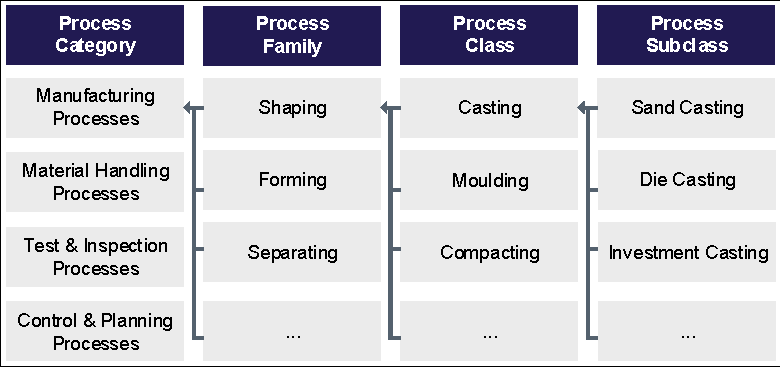
\includegraphics[width=.7\textwidth, trim=2 2 2 2, clip]{mainmatter/researchResults/figures/clsfScheme.pdf}
  \caption[Partially expanded overview of the consolidated classification scheme.]
  {Partially expanded consolidated overview of the classification scheme, focusing on the ``shaping'' process family and ``casting'' process class.
  Adapted from \parencite{SorensenCMS2018}.}\label{fig:clsfScheme}
\end{figure}
It consists of four levels (category, family, class, and subclass), adopting a structure similar to the one presented by \textcite{Ashby2011}.
The classification scheme has been modelled using Protégé~\parencite{Musen2015} and made available as an OWL file\footnote{\href{https://github.com/Firebrazer/ProdProcClass}{github.com/Firebrazer/ProdProcClass}}.
In total, the covered categories, families, classes, and subclasses comes to:
\begin{itemize}
  \item 4 process categories
  \item 16 process families
  \item 53 process classes
  \item 232 process subclasses
\end{itemize}

Manufacturing processes add ``form'' utility to workpieces, changing their shape or make-up.
It consists of six process families: shaping, forming, separating, change material properties, joining, and surface treatment.
Each process family is broken down another two times, each containing six to nine process classes, and each class listing up to ten subclasses.

Material handling processes add ``time'' and ``place'' utility by making sure a workpiece is at a specified location at the right time.
The material handling category consists of four process families: transport, storage(hold), handling, and unit load formation.
Focusing on processes occurring within the manufacturing system themselves, the transport and storage(hold) families were omitted from the study, as they occur between or outside manufacturing systems.
The handling and unit load formation families each consist of four classes with up to nine subclasses per class.

Focus for the study is on manufacturing and material handling processes, as such, the two remaining process categories (control \& planning and test \& inspection) have been left relatively unexplored during the study.
Control and planning processes manage, balance, and facilitate the utility provided by other processes, but does not strictly provide ``form'', ``time'' or ``place'' utility.
It contains three process families: business planning and control, manufacturing operations and control, and line control.

On the basis that the test and inspection processes provide a form of ``information'' utility rather than ``time'' and ``place'', they are separated from material handling and given their own category instead.
They capture and communicate various types of information related to workpieces.
This category is broken down into three families: inspection, functional test, and performance test.

\subsubsection*{Conclusions}
Based on a review and consolidation of production process classifications, taxonomies, and ontologies, a consolidated production process classification scheme has been created.
It groups processes into four categories based on the type of utility they add to a workpiece, further breaking down the categories into families, classes, and subclasses based on the characteristics of each process.
The process classification scheme is intended to facilitate consistent data collection on, and comparison of, existing manufacturing systems within a company.
This is done with the express purpose of identifying \gls{glos:cmmnlty} and \gls{glos:platformCand}s across manufacturing systems to enable platform development and standardisation of assets.

\subsection{Implications}
The classification scheme can be used to describe manufacturing systems based on the processes they perform in a consistent manner.
With a consistent and coherent classification of processes carried out by manufacturing systems, there is a potential for application of optimisation methods and algorithms to identify platform candidates, similarly to how \textcite{Kashkoush20161} form product families.
Using the individually distinguishable symbols presented in VDI 2860 to map or describe manufacturing systems can also facilitate rapid digitalisation of manually collected data, and generally speed up the process of comparing multiple manufacturing systems.

The classification scheme is expandable, as additional classes and subclasses can be added, should it prove necessary.
This may be needed when it comes to functional and performance tests, as some companies can have very specific tests that do not make sense to include or break down in a generic process classification scheme, \eg{} a ``final test'' process covering a number of very specific tests.
To recap, the outcome and contributions of the paper are:
\begin{enumerate}
  \item A consolidated process classification scheme covering manufacturing, material handling, planning, control, test, and inspection processes.
  \item A foundation upon which commonality can be identified across manufacturing systems, independently of physical means and solutions.
  \item An increased understanding of production processes and technology enabling them.
\end{enumerate}